% Section: Using Abisko
% Latex file for the MPI Course at HPC2N Umea 
%    Elaborated by P. Ojeda
%

\section{R/Matlab}

%%%%%%%%%%%%%%%%% NEW  SLIDE
\begin{frame}[fragile]
	\frametitle{R/Matlab}
\begin{itemize}
\item R is installed on Abisko and Kebnekaise. The MPI version
is only available on Kebnekaise. 

\item If additional modules are required, they can be installed 
locally. 

\item Regarding Matlab, one needs an initial setup (.matlab file)

\item Both serial and parallel versions of Matlab are available
on Abisko and Kebnekaise.

\item Kebnekaise supports the GPU version.
\end{itemize}

\end{frame}

\section{Accelerating applications}

%%%%%%%%%%%%%%%%% NEW  SLIDE
\begin{frame}[fragile]
	\frametitle{Matrix multiplication code (serial)}
{\small 
        \begin{verbatim}             
      do j=1,N
         do i=1,N
            do k=1,N
                p(i,j) = p(i,j) + v1(i,k)* v2(k,j)
            enddo
         enddo
      enddo
        \end{verbatim}
}
\end{frame}


%%%%%%%%%%%%%%%%% NEW  SLIDE
\begin{frame}[fragile]
	\frametitle{Matrix multiplication code (OpenMP)}
{\small 
        \begin{verbatim}             
!$omp parallel do private(i,j,k) shared(p,v1,v2) collapse(2)
      do j=1,N
         do i=1,N
            s=0.0d0
!$omp simd 
            do k=1,N
                s = s + v1(i,k)* v2(k,j)
            enddo
!$omp end simd
            p(i,j) = s
         enddo
      enddo
!$omp end parallel do
        \end{verbatim}
}
\end{frame}

%%%%%%%%%%%%%%%%% NEW  SLIDE
\begin{frame}[fragile]
	\frametitle{Matrix multiplication code (offload GPU)}
{\small 
        \begin{verbatim}             
!$omp target map(tofrom:p) map(to:v1,v2)
!$omp parallel do collapse(2) private(i,j,k,s)
      do j=1,N
         do i=1,N
            s=0.0d0
!$omp simd 
            do k=1,N
                s = s + v1(i,k)* v2(k,j)
            enddo
!$omp end simd
            p(i,j) = s
         enddo
      enddo
!$omp end parallel do
!$omp end target
        \end{verbatim}
}
\end{frame}





\section{Molecular Dynamics}
%%%%%%%%%%%%%%%%% NEW  SLIDE
\begin{frame}
	\frametitle{Long-range interactions}
\begin{columns}
	\column[T]{5cm}
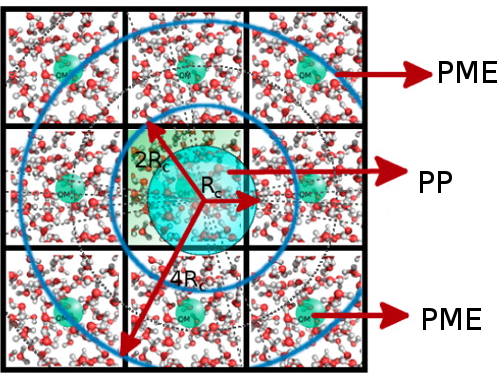
\includegraphics[width=5cm]{images/pppme.png}

{\tiny adapted from JCTC,10,134 (2014)}
	\column[T]{5cm}
	\begin{itemize}
		\item	particle-particle interactions are solved in real space (80$\%$)
		\item	PME contribution is solved in reciprocal space (20$\%$)
	\end{itemize}
\end{columns}
\end{frame}
%
%%%%%%%%%%%%%%%%% NEW  SLIDE
\begin{frame}
	\frametitle{Workflow MD code}
        \begin{center}
\includegraphics[width=6cm]{images/md_interactions_scheme.png}
        \end{center}

\end{frame}
%
%%------------------  NEW SUBSECTION ------------------
%%%%%%%%%%%%%%%%% NEW  SLIDE
\section{AMBER}

%%%%%%%%%%%%%%%%% NEW  SLIDE
\begin{frame}[fragile]
	\frametitle{AMBER}
{\small 
        \begin{verbatim}             
$module spider amber
-------------------------------------------------------------------------------------------------------------------------------------------------------------------------------------------------------------------
  Amber:
-------------------------------------------------------------------------------------------------------------------------------------------------------------------------------------------------------------------
    Description:
      Amber (originally Assisted Model Building with Energy Refinement) is software for performing molecular dynamics and structure prediction. - Homepage: http://ambermd.org/amber.html 

     Versions:
        Amber/16-AmberTools-16-patchlevel-20-7-hpc2n (GPU)
        Amber/16-AmberTools-16-patchlevel-20-7

        \end{verbatim}
}
\end{frame}

%%%%%%%%%%%%%%%%% NEW  SLIDE
\begin{frame}[fragile]
	\frametitle{AMBER batch script (Sander)}
        \begin{verbatim}             
#!/bin/bash
#SBATCH -A <Your-Project-Here>
#SBATCH -n 8
#SBATCH --time=01:00:00

module load icc/2017.1.132-GCC-5.4.0-2.26  impi/2017.1.132 ifort/2017.1.132-GCC-5.4.0-2.26
module load Amber/16-AmberTools-16-patchlevel-20-7

srun sander.MPI -ng 8 -groupfile equilibrate.groupfile
        \end{verbatim}

\end{frame}

%%%%%%%%%%%%%%%%% NEW  SLIDE
\begin{frame}[fragile]
	\frametitle{AMBER batch script (Pmemd)}
        \begin{verbatim}             
#!/bin/bash
#SBATCH -A <Your-Project-Here>
#SBATCH -n 96
#SBATCH --ntasks-per-node=48
#SBATCH --time=01:00:00

module load icc/2017.1.132-GCC-5.4.0-2.26  impi/2017.1.132 \
ifort/2017.1.132-GCC-5.4.0-2.26
module load Amber/16-AmberTools-16-patchlevel-20-7

srun pmemd.MPI -O -i 02_heat.in -o 02_heat.out -p \
ala_tri.prmtop -c 01_min.rst -r 02_heat.rst -x 02_heat.nc
        \end{verbatim}

\end{frame}

%%%%%%%%%%%%%%%%% NEW  SLIDE
\begin{frame}[fragile]
	\frametitle{AMBER batch script (single GPU engine)}
        \begin{verbatim}             
#!/bin/bash
#SBATCH -J Amber
#SBATCH -A <Your-Project-Here>
#SBATCH -n 1
#SBATCH --gres=gpu:k80:1
#SBATCH --time=1:00:00

module load icc/2017.1.132-GCC-5.4.0-2.26 ifort/2017.1.132-GCC-5.4.0-2.26
module load CUDA/8.0.44
module load Amber/16-AmberTools-16-patchlevel-20-7-hpc2n
pmemd.cuda -O -i mdinfile -o mdoutfile -c inpcrdfile \
-p prmtopfile -r restrtfile
        \end{verbatim}

\end{frame}

\begin{frame}
	\frametitle{AMBER performance 158944 atoms system}
        \begin{center}
		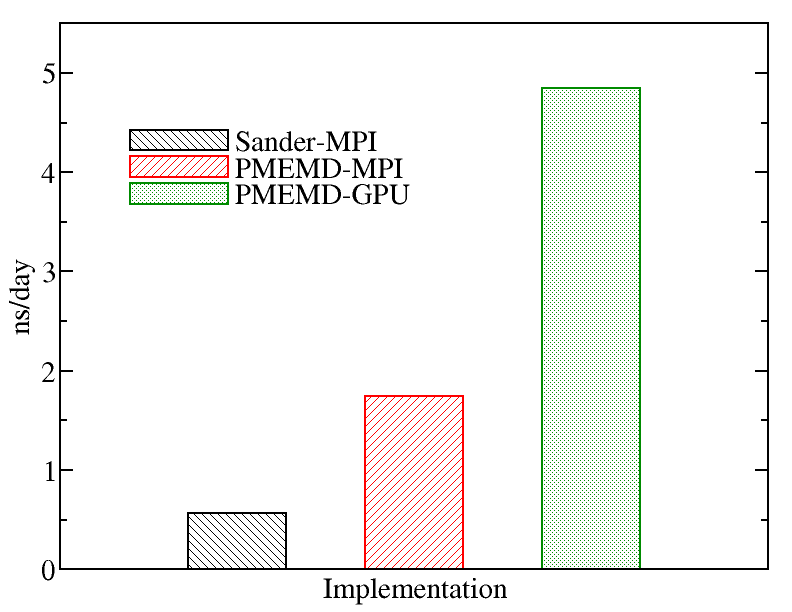
\includegraphics[width=8cm]{images/profiling_amber.png}
        \end{center}
\end{frame}

%%%%%%%%%%%%%%%%% NEW  SLIDE
\section{NAMD}


%%%%%%%%%%%%%%%%% NEW  SLIDE
\begin{frame}[fragile]
	\frametitle{NAMD}
{\small 
        \begin{verbatim}             
$module spider namd
------------------------------------------------------------------------------------------------------------------------------------------------------------------------------------------------------------------
  NAMD:
-------------------------------------------------------------------------------------------------------------------------------------------------------------------------------------------------------------------
    Description:
      NAMD is a parallel molecular dynamics code designed for high-performance simulation of large biomolecular systems. - Homepage: http://www.ks.uiuc.edu/Research/namd/ 

     Versions:
        NAMD/2.12-mpi
        NAMD/2.12-nompi (GPU support)
        \end{verbatim}
}
\end{frame}

\begin{frame}[fragile]
	\frametitle{NAMD 6 cores}
  
        \begin{verbatim}             
#!/bin/bash
#SBATCH -A SNICXXXX-Y-ZZ
#SBATCH -t 00:10:00
#SBATCH -N 1
#SBATCH -c 6

module add icc/2017.1.132-GCC-6.3.0-2.27  impi/2017.1.132
module add NAMD/2.12-nompi

namd2 +p6 config_file > output_file
        \end{verbatim}

\end{frame}

\begin{frame}[fragile]
	\frametitle{NAMD all cores}
  
        \begin{verbatim}             
#!/bin/bash
#SBATCH -A SNICXXXX-Y-ZZ
#SBATCH -t 00:10:00
#SBATCH -N 1
#SBATCH -c 28

module add icc/2017.1.132-GCC-6.3.0-2.27 impi/2017.1.132
module add NAMD/2.12-nompi

namd2 +p28 config_file > output_file
        \end{verbatim}

\end{frame}


\begin{frame}[fragile]
	\frametitle{NAMD on GPUs}
  
        \begin{verbatim}             
#!/bin/bash
#SBATCH -A SNICXXXX-Y-ZZ
#SBATCH -t 00:10:00
#SBATCH -N 1
#SBATCH -c 28
#SBATCH --exclusive
#Ask for 2 GPU cards
#SBATCH --gres=gpu:k80:2

module add GCC/5.4.0-2.26  CUDA/8.0.61_375.26  OpenMPI/2.0.2
module add NAMD/2.12-nompi

namd2 +p28 config_file > output_file
        \end{verbatim}

\end{frame}



\begin{frame}[fragile]
	\frametitle{NAMD more than 1 node}
  
        \begin{verbatim}             
#!/bin/bash
#SBATCH -A SNICXXXX-Y-ZZ
#SBATCH -t 00:10:00
#SBATCH -N 2
#SBATCH -n 2
#SBATCH -c 28
#SBATCH --exclusive

module add GCC/6.3.0-2.27  OpenMPI/2.0.2
module add NAMD/2.12-mpi

srun -N 2 -n 2 namd2 +ppn 27 config_file > output_file
        \end{verbatim}

\end{frame}

\begin{frame}
	\frametitle{NAMD performance 23074 atoms system}
        \begin{center}
		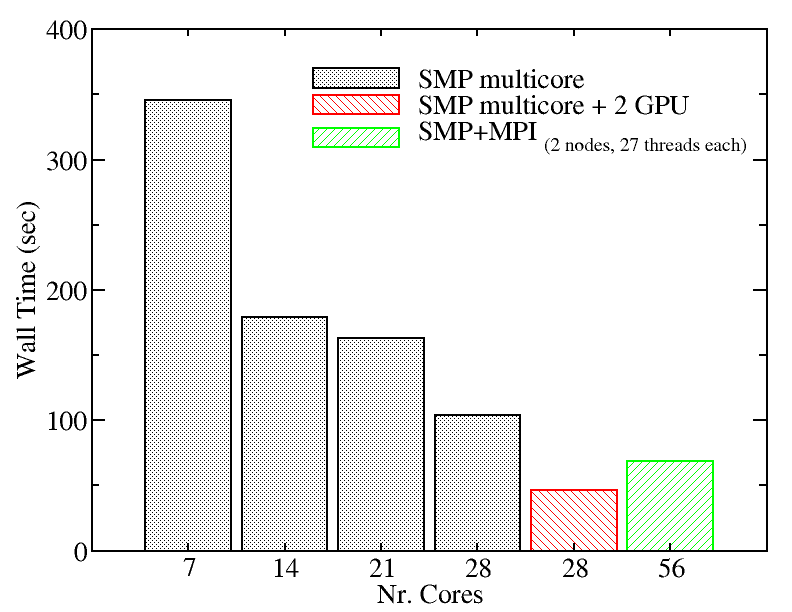
\includegraphics[width=8cm]{images/profiling_namd.png}
        \end{center}
\end{frame}


\begin{frame}
	\frametitle{NAMD performance 158944 atoms system}
        \begin{center}
		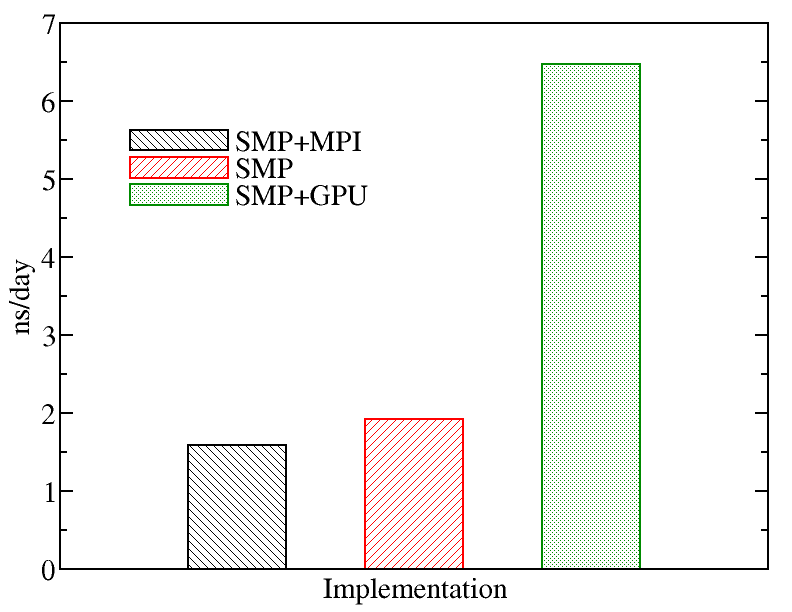
\includegraphics[width=8cm]{images/profiling_namd2.png}
        \end{center}
\end{frame}



%%------------------  NEW SUBSECTION ------------------
%%%%%%%%%%%%%%%%% NEW  SLIDE
\section{GROMACS}

%%%%%%%%%%%%%%%%% NEW  SLIDE
\begin{frame}[fragile]
	\frametitle{GROMACS}
{\small 
        \begin{verbatim}             
$module spider gromacs
---------------------------------------------------------
  GROMACS:
---------------------------------------------------------
    Description:
      GROMACS is a versatile package to perform molecular 
      systems with hundreds to millions of particles. - 

     Versions:
        GROMACS/5.1.4-hybrid
        GROMACS/5.1.4-mt
        GROMACS/2016-hybrid
        GROMACS/2016-mt

----------------------------------------------------------------------------------------------------------------------------
  For detailed information about a specific "GROMACS" 
  For example:

        \end{verbatim}
}
\end{frame}


%%%%%%%%%%%%%%%%% NEW  SLIDE
\begin{frame}[fragile]
	\frametitle{GROMACS}
  
        \begin{verbatim}             
$module spider GROMACS/2016-hybrid 
------------------------------------------------------------------------------------------------------------------------------------------------------------------------------------------------------------------------------------------------------------------
  GROMACS: GROMACS/2016-hybrid
------------------------------------------------------------------------------------------------------------------------------------------------------------------------------------------------------------------------------------------------------------------
 Description:
   GROMACS is a versatile package to ... 
   Homepage: http://www.gromacs.org 

   You will need to load all module(s) on any one of 
   the lines below before the "GROMACS/2016-hybrid" ...

   GCC/5.4.0-2.26  CUDA/8.0.44  OpenMPI/2.0.1
   GCC/6.2.0-2.27  OpenMPI/2.0.1

        \end{verbatim}

\end{frame}


%%%%%%%%%%%%%%%%% NEW  SLIDE
\begin{frame}[fragile]
	\frametitle{GROMACS batch script}
        \begin{verbatim}             
#!/bin/bash
#SBATCH -A ~SNICYYYY-XX-NN
#SBATCH -t 01:00:00
#SBATCH -n 12
#SBATCH -c 7
#SBATCH --gres=gpu:k80:2
#SBATCH -p batch
module add CUDA/8.0.44   GCC/5.4.0-2.26   
module add OpenMPI/2.0.1 GROMACS/2016-hybrid
mdargs="-ntomp $SLURM_CPUS_PER_TASK"
mpirun -np $SLURM_NTASKS gmx_mpi mdrun $mdargs \ 
-dlb yes  -v -deffnm npt
        \end{verbatim}
\end{frame}



%%%%%%%%%%%%%%%%% NEW  SLIDE
\begin{frame}[fragile]
	\frametitle{GROMACS output}
  
        \begin{verbatim}             
    
Running on 3 nodes with total 84 cores, 
84 logical cores, 12 compatible GPUs
  Cores per node:           28                                          
  Logical cores per node:   28                 
  Compatible GPUs per node:  4                 
  All nodes have identical type(s) of GPUs  

        \end{verbatim}

\end{frame}
%%%%%%%%%%%%%%%%% NEW  SLIDE

\begin{frame}
	\frametitle{GROMACS performance 100K atoms}
        \begin{center}
		\includegraphics[width=8cm]{images/data_kebne.eps}
        \end{center}
\end{frame}

%%%%%%%%%%%%%%%%% NEW  SLIDE
\begin{frame}
	\frametitle{GROMACS performance 158944 atoms system}
        \begin{center}
		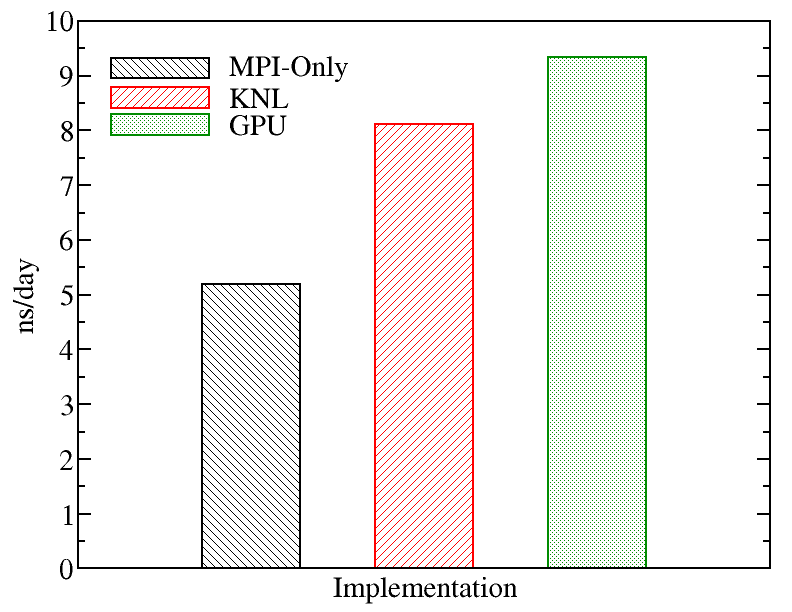
\includegraphics[width=8cm]{images/profiling_gromacs.png}
        \end{center}
\end{frame}


\begin{frame}
	\frametitle{Profiling Tools SCALASCA/GROMACS}
        \begin{center}
		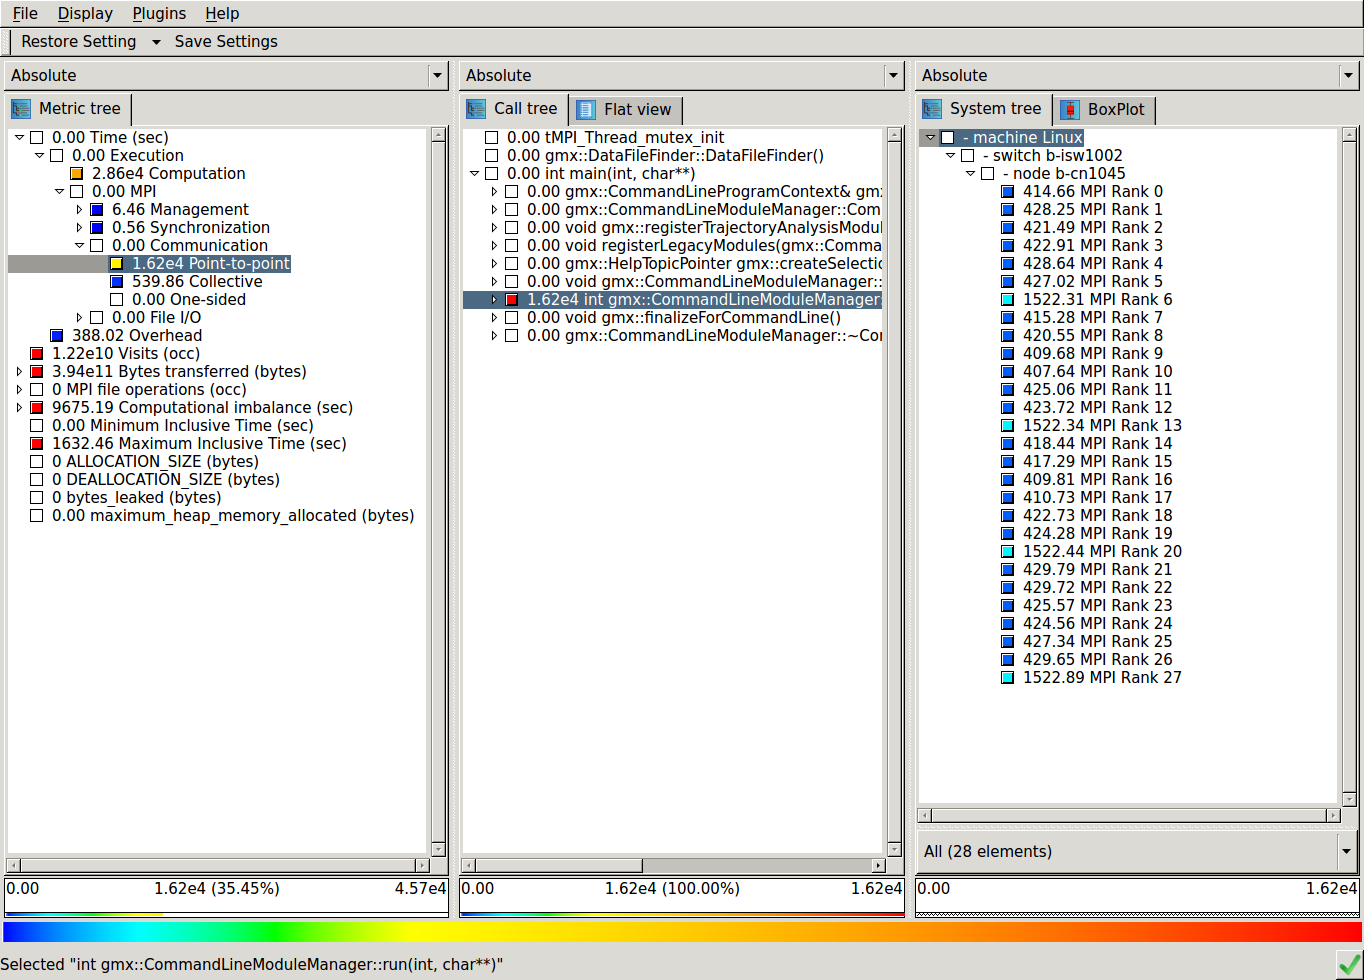
\includegraphics[width=9cm]{images/cube_gromacs.png}
        \end{center}
\end{frame}



\section{CHARMM}
%%%%%%%%%%%%%%%%% NEW  SLIDE
\begin{frame}[fragile]
	\frametitle{DOMDEC CHARMM}
  
        \begin{verbatim}             
module add GCCcore/5.4.0    
module add GCC/5.4.0-2.26   
module add CUDA/8.0.44

./install.com gnu M fftw  domdec_gpu
        \end{verbatim}

\end{frame}

%%%%%%%%%%%%%%%%% NEW  SLIDE
\begin{frame}[fragile]
	\frametitle{DOMDEC CHARMM}
  
        \begin{verbatim}             
<domdec_dr_common> No direct/recip split, using all nodes on both                                                                                                                               
Number of CUDA devices found 4
Using CUDA driver version 8000
Using CUDA runtime version 8000
Node 0 uses CUDA device 3 Tesla K80 with CUDA_ARCH 350
Intel CPU | Using CUDA version of non-bonded force loops and SSE elsewhere
Initializing DOMDEC with NDIR =   1  1  1  
Number of threads per MPI node =  28 
Dynamic Load Balancing disabled
Splitting recip cores into (y by z):   1 by    1
        \end{verbatim}

\end{frame}

%%%%%%%%%%%%%%%%% NEW  SLIDE
\begin{frame}[fragile]
	\frametitle{batch script DOMDEC CHARMM}
  
        \begin{verbatim}             
#!/bin/bash
#SBATCH -A staff
#SBATCH -J G2016-gpu
#SBATCH -t 12:00:00
#SBATCH -n 1         ##number of mpis
#SBATCH -c 28         ##number of openmp threads
#SBATCH --gres=gpu:k80:2
#SBATCH -p batch
module add GCCcore/5.4.0 GCC/5.4.0-2.26 CUDA/8.0.44   
mpirun -np $SLURM_NTASKS -x OMP_NUM_THREADS=28 \
 --bind-to none /home/p/pojedama/pfs/c42a1/ \
exec/gnu_M/charmm < m.inp > out.dat
        \end{verbatim}

\end{frame}


%%%%%%%%%%%%%%%%% NEW  SLIDE

\begin{frame}
	\frametitle{Profiling Tools SCALASCA/CHARMM}
        \begin{center}
		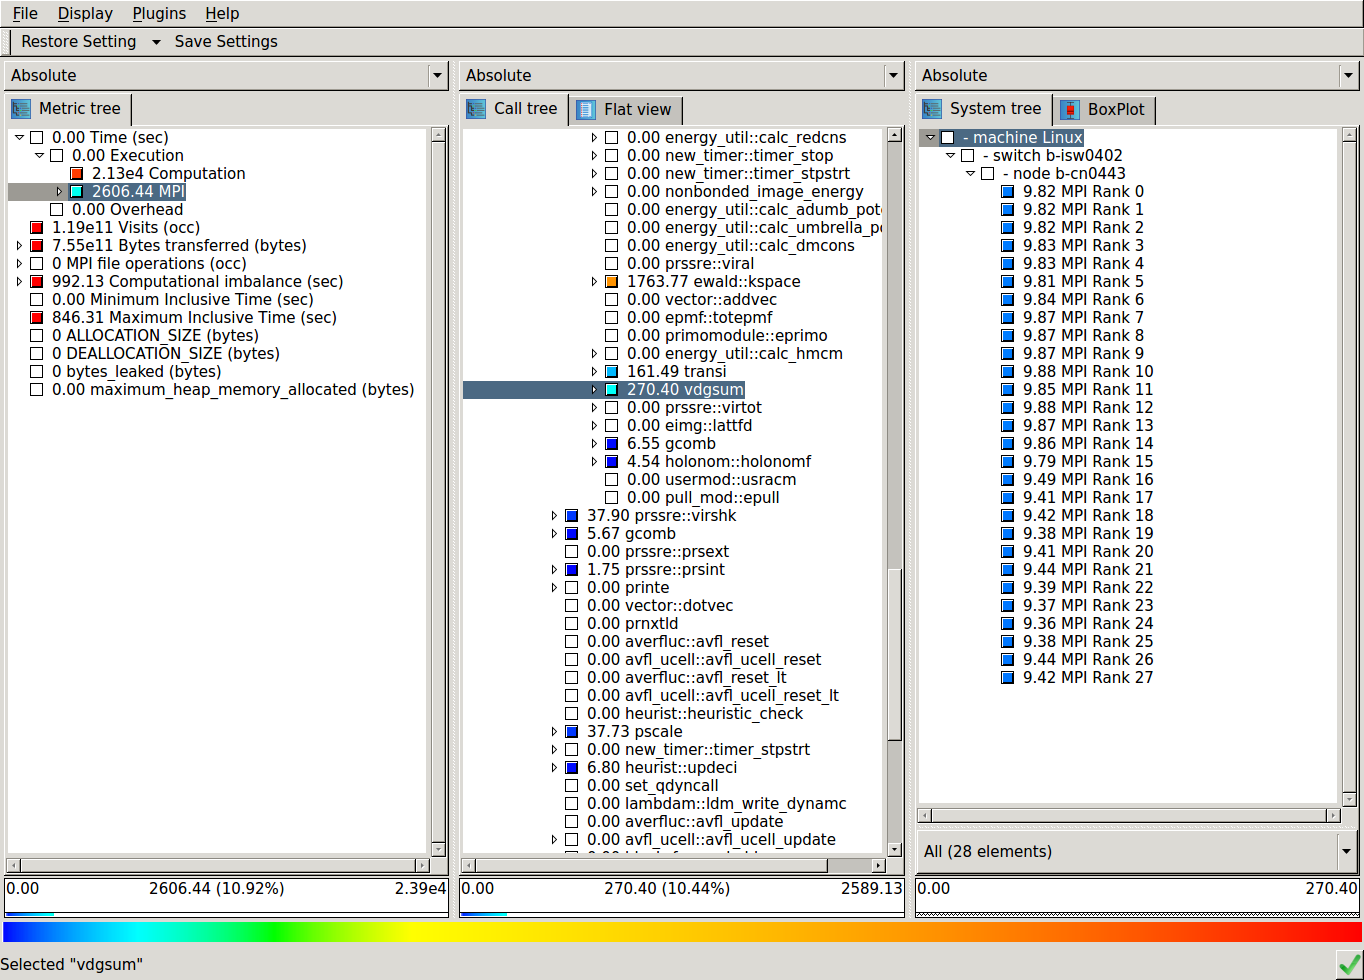
\includegraphics[width=9cm]{images/cube_charmm.png}
        \end{center}
\end{frame}

%%%%%%%%%%%%%%%%% NEW  SLIDE

\begin{frame}
	\frametitle{Scaling behavior modern MD software}
        \begin{center}
		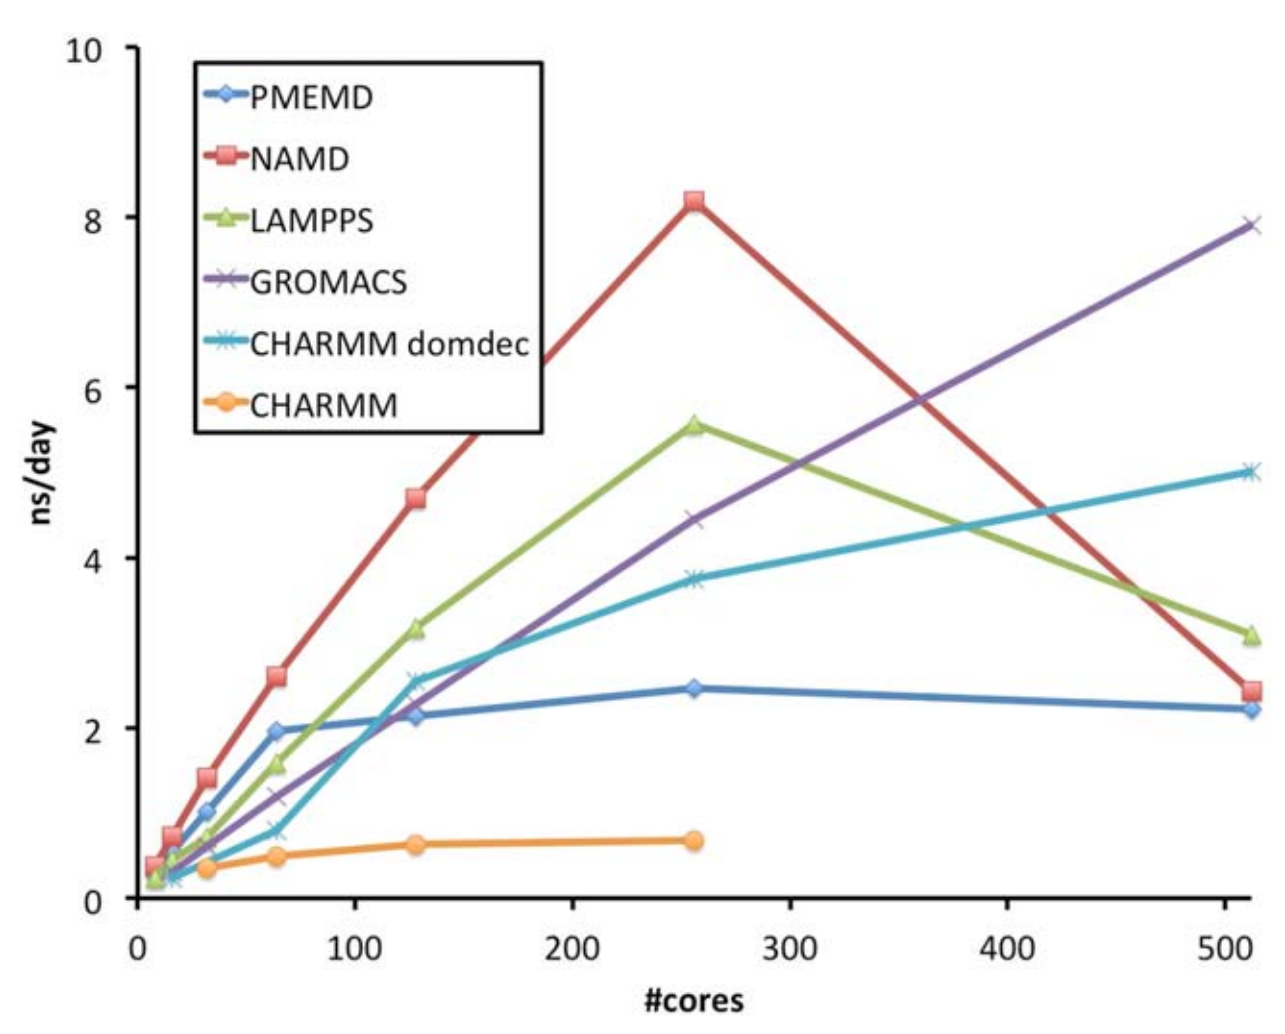
\includegraphics[width=8cm]{images/software_scaling.png}
        \end{center}

{\tiny
source: hEGFR with 465,404 atoms. JCC, 35, 406 (2014).
}
\end{frame}



\section{GAUSSIAN}
%%%%%%%%%%%%%%%%% NEW  SLIDE
\begin{frame}[fragile]
	\frametitle{batch script GAUSSIAN}
  
        \begin{verbatim}             
#!/bin/bash
#SBATCH -A staff
#SBATCH -N 1
#SBATCH -c 28
#SBATCH --exclusive
#SBATCH --gres=gpu:k80:2
#SBATCH --time=00:10:00

module add gaussian/16.A.03-AVX2
# Assume that the job file are located in the submit directory
g16.set-cpu+gpu-list input.com
time g16 input

        \end{verbatim}

\end{frame}

%%%%%%%%%%%%%%%%% NEW  SLIDE
\begin{frame}[fragile]
	\frametitle{GAUSSIAN on GPUs}
  
Initial input file:
{\tiny
        \begin{verbatim}             
$more input_bk.com 
%chk=geom_optim.chk
%mem=16GB
#UB3LYP/6-31+G(d) OPT=(ModRedun) SCF=(MaxCycle=256) pop=none NoSymm

45 atoms structure, RESP

+5 15
O       3.744336        -1.126487       6.111505
P       2.893853        -1.251776       4.246949
O       4.150424        -3.154051       4.078061
        \end{verbatim}
}

Corrected input file:

{\tiny
        \begin{verbatim}             
$more input.com 
%cpu=0,1,2,3,4,5,6,7,8,9,10,11,12,13,14,15,16,17,18,19,20,21,22,23,24,25,26,27
%gpucpu=0-3=0,7,14,21
%chk=geom_optim.chk
%mem=16GB
#UB3LYP/6-31+G(d) OPT=(ModRedun) SCF=(MaxCycle=256) pop=none NoSymm

45 atoms structure, RESP

+5 15
O       3.744336        -1.126487       6.111505
P       2.893853        -1.251776       4.246949
O       4.150424        -3.154051       4.078061
        \end{verbatim}
}


\end{frame}

\section{EasyBuild}
%%%%%%%%%%%%%%%%% NEW  SLIDE
\begin{frame}[fragile]
	\frametitle{Installing your own software}
  
\begin{itemize}

\item We use EasyBuild to install software on Abisko/Kebnekaise.

\item You can install your own software on your local directory using EasyBuild
and make it available for later use.





\end{itemize}

\end{frame}

